\section{Realization}
\label{sec:realization}
%Focus generale sulle tecnologie utilizzate
In this section, we outline the technical aspects concerning the realization of our approach. Therefore we first present the enabler technologies through which we instantiate the design principles presented in \cref{sec:design}. After that, we discuss the interaction workflow between the instantiated technologies. Finally, we show the implementation details.

\subsection{Deployment}
As follows, we bridge the gap between high-level system architecture and its practical realization. \cref{fig:deployment_diagram} depicts a \textit{UML deployment diagram} \cite{koch2002expressive} that aims to help with understanding the instantiated infrastructure. 

In our solution, we make a differentiation between the technologies designated for mining, denoted as \Compo{Miner Machine}s, and those specifically associated with provisioners, identified as \Compo{Provisioner Machine}s. To enhance clarity, we maintain the separation of these \textit{devices} in the accompanying diagram. However, organizations have the flexibility to opt for integrated technologies that incorporate both mining and provisioning functionalities. Using our motivating scenario as an example, the \Actor{Hospital} can be equipped with machines aimed for both mining and provisioning, while the \Actor{Specialized clinic} can make use of separate devices. We included the \texttt{Log Recorder}, the \texttt{Log Provider}, and \texttt{Secure Miner} (already discussed in \cref{sec:design}) as abstract \textit{components} of the diagram, whose manifestation are described as follow. 

\Compo{Provisioner Machine}s encompasses \Compo{Log Recorder}s and \Compo{Log Provider}s incorporating their core functionalities aimed at generating and transmitting event logs. Within the organizational context, we manifest the \Compo{Log Recorder} in the Process Aware Information System (\Compo{PAIS}), which plays a crucial role in managing various business processes, including accounting and resource management \cite{Dumas.etal/2018:FundamentalsofBPM}. In our motivating scenario, the \Actor{Hospital} and the other provisioner parties generate the traces Alice and Bob through this type of systems.
\begin{figure}[t]
	\centering
	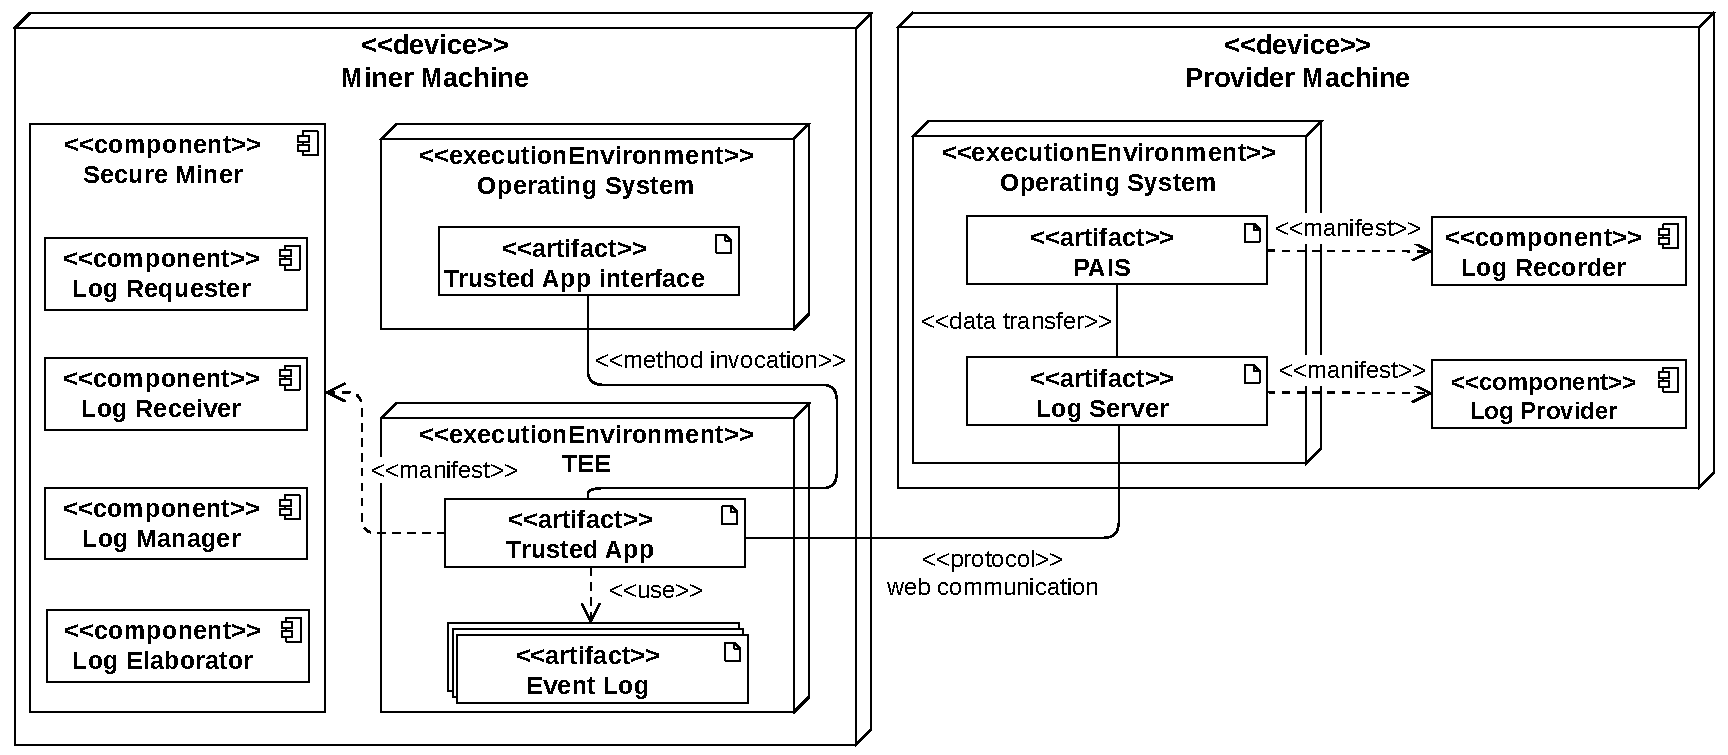
\includegraphics[width=1\linewidth]{content/figures/deploymentdiagram3.pdf}
	\caption{UML deployment diagram.}
	\label{fig:deployment_diagram}
\end{figure}
In our solution, the \Compo{PAIS} grants access to the \Compo{Log Server}, enabling it to retrieve event logs. The \Compo{Log Server}, on the other hand, embody the functionalities of the \Compo{Log Provider}, implementing web services aimed at handling remote data requests and providing event log data to miners. The \Actor{Hospital}, the \Actor{Specialized Clinic} and the \Actor{Pharmaceutical Company} of our running example employes \Compo{Log Servers} adhering to established web standards such as HTTP\footnote{\url{https://www.w3.org/Protocols/rfc2616/rfc2616.html}}, FTP\footnote{\url{https://www.w3.org/Protocols/rfc959/}}, and Goopher\footnote{\url{https://datatracker.ietf.org/doc/html/rfc1436}}. Both the \Compo{PAIS} and \Compo{Log Server} run on the top the \Compo{Operating System} of the \Compo{Provisioner Machine}.

The \Compo{Miner Machine} is characterized by two distinct \textit{execution environments}: the \Compo{Operating System} and the Trusted Execution Environment (\Compo{TEE}). \Compo{TEE}s establish an isolated context separate from the normal \Compo{Operating System}, safeguarding code and data through hardware-based encryption mechanisms. This technology relies on specialized components of the \Compo{Miner Machine}'s CPU capable of managing encrypted data within a reserved section of RAM \cite{TEEHERE}. We leverage the security guarantees provided by \Compo{TEE}s to isolate a \Compo{Trusted App} responsible for fulfilling the functions of the \Compo{Secure Miner} and its associated subcomponents. The \Compo{Trusted App} consolidates the logic required for generating verifiable data requests, receiving external event logs, securely storing them within the \Compo{TEE}, and executing process mining algorithms. All procedures executed by the \Compo{Trusted App} are tamper-proof. The \Compo{TEE} ensures the integrity of the \Compo{Trusted App} code, protecting it against malicious manipulations and unauthorized access by entities operating within the \Compo{Operating System}. Additionally, we utilize the isolated environment of \Compo{TEE}s to securely store event log data (e.g., the traces of Alice and Bob of our example) from provisioner organizations within the \Compo{Miner Machine}. The \Compo{TEE} safeguards this sensitive information alongside a unique asymetric key couple used for attestation purposes (i.e., public and private keys), preventing exposure to the \Compo{Operating System}. Access to data located in the \Compo{TEE} is restricted solely to the \Compo{Trusted App}. Users interact with the \Compo{Trusted App} through the \Compo{Trusted App Interface}, which serves as the exclusive communication channel. The \Compo{Trusted App} offers secure methods, invoked by the \Compo{Trusted App Interface}, for safely receiving information from the \Compo{Operating System} and outsourcing the results of computations, maintaining a high level of data security.

In the next subsection, we elucidate the interaction between the newly introduced technologies.
\begin{comment}
\begin{figure}[t]
\centering
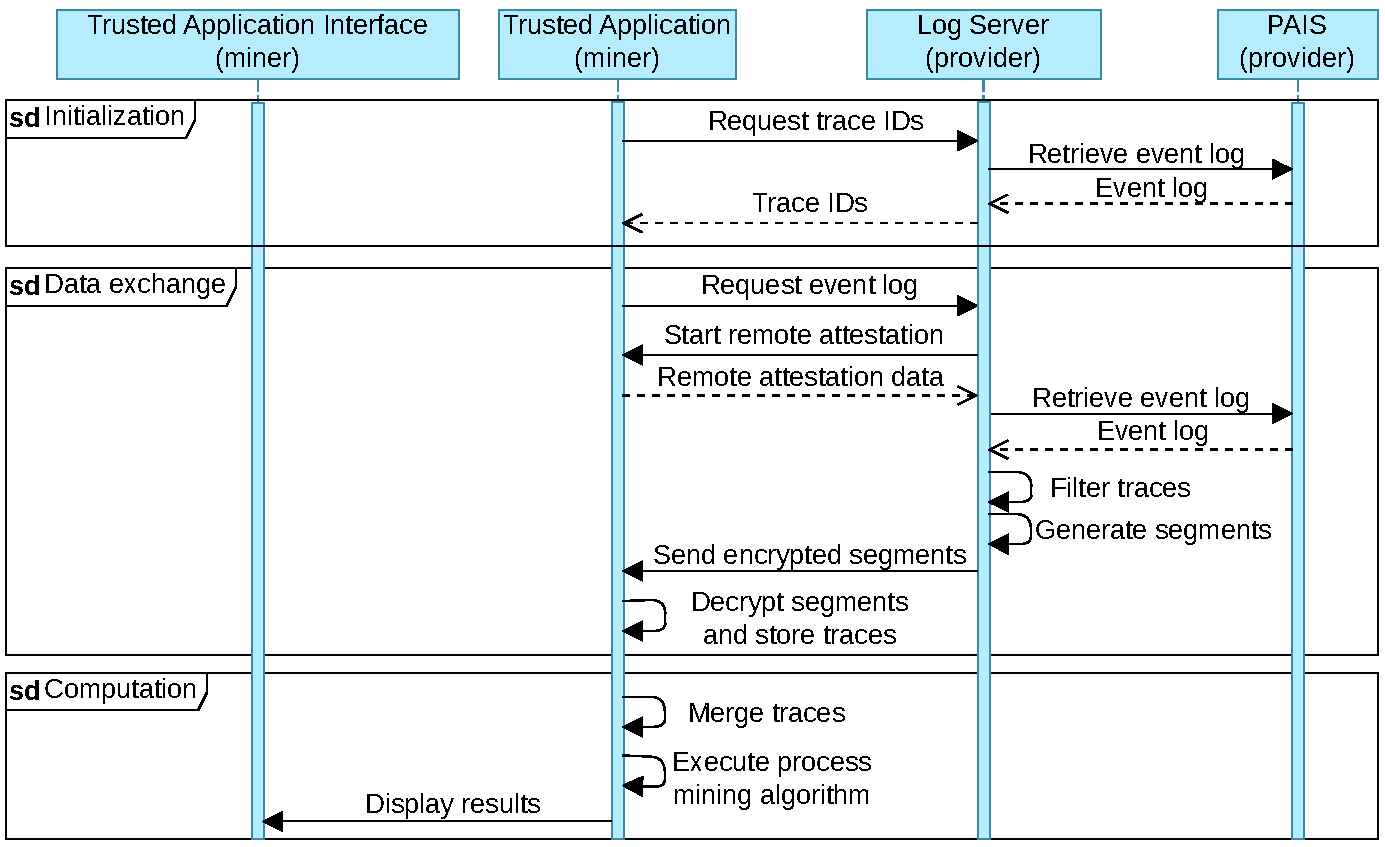
\includegraphics[width=0.9\linewidth]{content/figures/sequencediagram.pdf}
\caption{UML sequence diagram.}
\label{fig:sequence_diagram}
\end{figure}
\end{comment}


\subsection{Workflow}

We separate the workflow into subsequent processes, namely \textit{initialization}, \textit{remote attestation}, \textit{data transmission}, and \textit{computation}. This sequence of activities is enacted by two principal entities: a \Compo{Miner Machine} and a variable number, denoted in as \texttt{n}, of \Compo{Provisioner Machines}. We depict each stage separately in \cref{fig:workflow} and \cref{fig:workflow2}.

\begin{figure}[t]
	\subfloat[][Initialization]{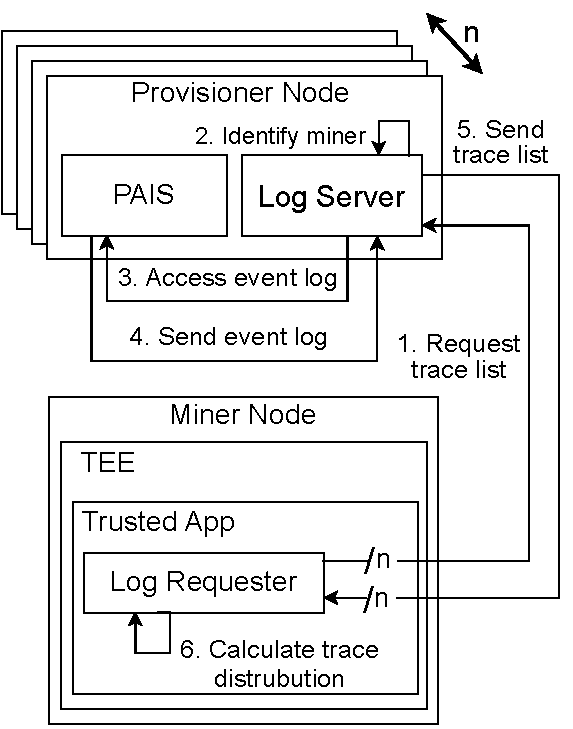
\includegraphics[width=0.29\linewidth]{content/figures/initializationworkflow.pdf}\label{fig:init}}\hfill
	\subfloat[][Remote Attestation]{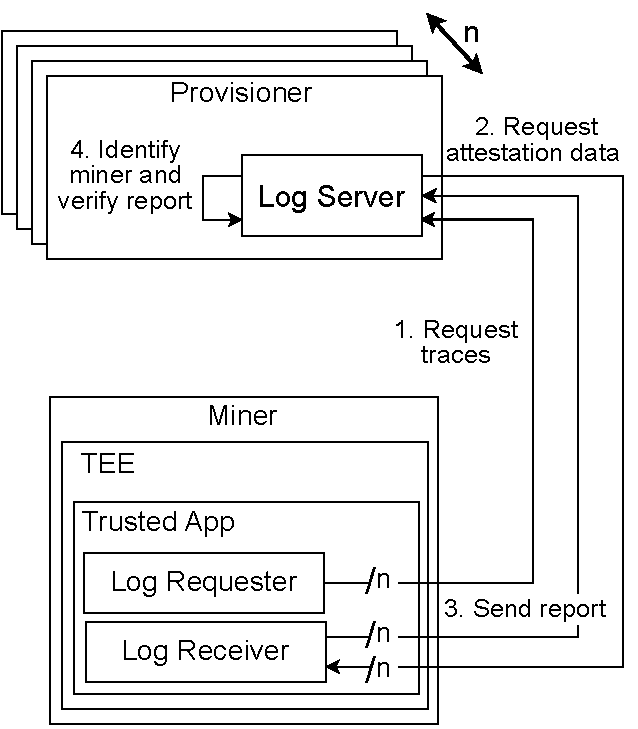
\includegraphics[width=0.32\linewidth]{content/figures/attestationworkflow.pdf}\label{fig:attestation}}\hfill
	\subfloat[][Data Transmission]{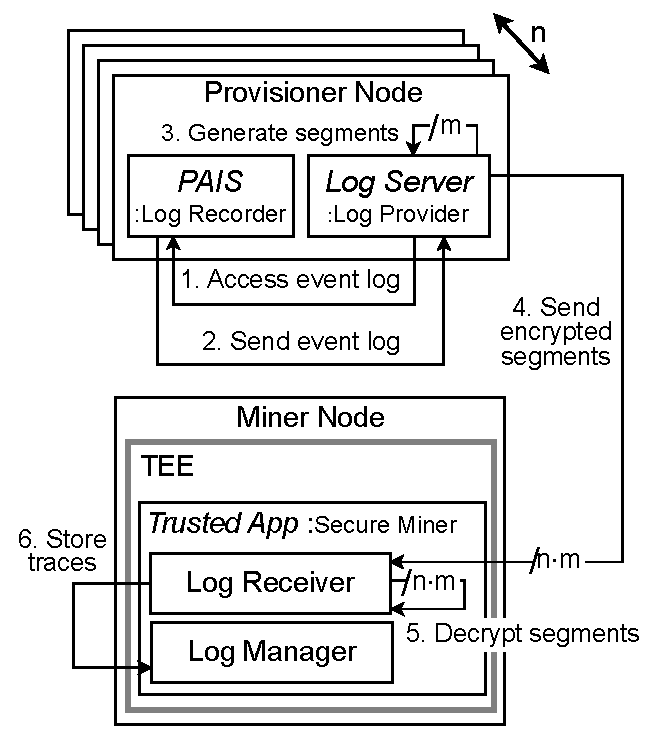
\includegraphics[width=0.33\linewidth]{content/figures/datatransmissionworkflow.pdf}\label{fig:transmission}}\hfill
	\caption{Schematization of the initialization, remote attestation and data transmission phase.}
	\label{fig:workflow}
\end{figure}
\textbf{Initialization.} The objective of the initialization stage is to inform the miner about the distribution of traces related to a business process among the \Compo{Provisioner Machines}, before the commencement of the computation. At the onset of this process, the \Compo{Log Requester} component within the \Compo{Trusted App} issues \texttt{n} requests to the Log Server components of the provisioners for the list of owned traces(\texttt{1}, in \cref{fig:init}). Following sender authentication (\texttt{2}), each \Compo{Log Server} retrieves the local event log from the \Compo{PAIS} (\texttt{3}, \texttt{4}) and subsequently responds to the \Compo{Log Requester} by providing a list of its associated traces(5). After collecting these \Compo{n} responses, the \Compo{Log Requester} delineates the distribution of traces. In the context of our motivating scenario, by the conclusion of the initialization phase, the miner gains knowledge that traces belonging Bob's process, specifically $T^H_{711}$ and $T^C_{711}$, are exclusively retained by the \Actor{Hospital} and the \Actor{Specialized Clinic}. In contrast, traces recording to Alice's process, denoted as $T^H_{312}$, $T^C_{312}$, and $T^S_{312}$, are scattered across all three organizations.

\begin{wrapfigure}[11]{r}{0.35\textwidth}
	\vspace{-2em}
	\centering
	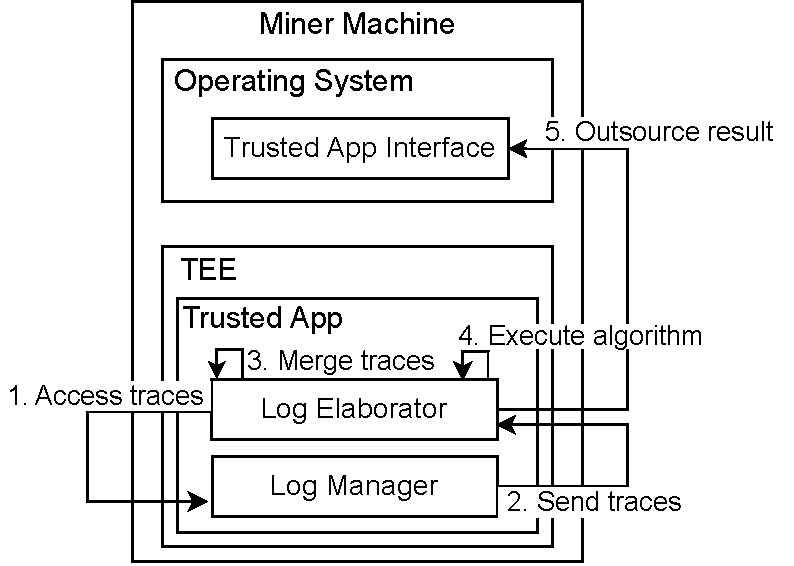
\includegraphics[width=1\textwidth]{content/figures/computationworkflow.pdf}
	\caption[A gull]{Schematization of the computation phase.}
	\vspace{-6pt}
	\label{fig:workflow2}
\end{wrapfigure}
\textbf{Remote Attestation.} The remote attestation serves the purpose of establishing trust between miners and provisioners in the context of fulfilling data requests. This procedure has a dual objective: (i) to furnish provisioners with compelling evidence that the data request for an event log originates from a \Compo{Trusted App} currently executing within a \Compo{TEE} (Trusted Execution Environment), and (ii) to confirm the precise nature of the \Compo{Trusted App} as an authentic \Compo{Secure Miner} software entity. Upon the initiation of a new log request by the \Compo{Log Requester} (\texttt{1}, in \cref{fig:attestation}), each of the \texttt{n} \Compo{Log Server}s commences the verification process by requesting the necessary information from the \Compo{Log Receiver} to conduct the attestation (\texttt{2}). Subsequently, the \Compo{Log Receiver} generates a report containing the measurement of the \Compo{Trusted App,} which is defined as the hash value of the combination of the code and initial data of the software. Once this report is signed using the attestation private key associated with the hardware of the \Compo{Miner Machine}, it is transmitted from the \Compo{Log Receiver} to the \Compo{Log Server}s (\texttt{3}). The \Compo{Log Server}s authenticate the miner and decrypt the report using its attestation public key (\texttt{4}). In this last step, the \Compo{Log Server}s undertake a comparison procedure in which they juxtapose the measurement found within the decrypted report against a predefined reference value associated with the source code of the \Compo{Secure Miner}.

\textbf{Data Transmission.} Once verified the trusted nature of the \Compo{Trusted App}, the \Compo{Log Servers} can proceed with the transmission of their traces. To accomplish this, each \Compo{Log Server} retrieves the event log from the \Compo{PAIS} (\texttt{1} and \texttt{2}, in \cref{fig:transmission}), and divides it into segments, resulting in \texttt{m} segments (\texttt{3}). Each of these segments contains a variable number of complete traces, with the cumulative size remaining within the threshold specified by the miner as a parameter of the initial request. As an illustrative example from our motivating scenario, the \Compo{Log Server} of the \Actor{Hospital} may structure the segmentation such that $T^H_{312}$ and $T^H_{711}$ reside within the same segment, whereas the \Actor{Specialized clinic} might have $T^S_{312}$ and $T^S_{711}$ in separate segments. Subsequently, the \texttt{n} \Compo{Log Server}s transmit their \texttt{m} encrypted segments to the \Compo{Log Receiver} of the \Compo{Trusted App} (\texttt{4}). The \Compo{Log Receiver}, in turn, decrypts each of the \texttt{n} • \texttt{m} responses (\texttt{5}) and securely stores the traces within the \Compo{TEE} through the \Compo{Log Manager} (\texttt{6}).

\textbf{Computation.} To start a computation routine, the \texttt{Trusted App} require all the provisioners to have delivered traces referring to the same process instances. For example, when $T^H_{312}$, $T^S_{312}$ and $T^C_{312}$ are all received by the \Compo{Trusted App}, the process instance of Alice is elegible as input for the computation. When this occurs, the \texttt{Trusted App} merges external traces with the owned one. Assembled traces are used as parameters of process mining algorithms executed by the \texttt{Trusted Application} that presents the computation results to the users via the \texttt{Trusted Application Interface}.








\subsection{Implementation}
\label{sec:implementation:details}
\todo[inline]{Punti da toccare: link git, intel sgx, EGo in golang, comunicazione trusted app - log server in HTTP, Heuristic Miner come algoritmo prof of concept Process Mining che genera Workflownet. Più coincisi il possibile.}
The proposed implementation integrates a trusted application within a secure execution environment, complemented by the inclusion of event logs to address the issue outlined in the motivating scenario. The source code is accessible at the following URL: \url{https://github.com/dave0909/TEExProcessMining/}. 

To realize the implementation of trusted applications, we employed EGo,\footnote{https://www.edgeless.systems/products/ego/} a framework designed for encoding trusted application in the Go\footnote{https://go.dev} programming language. Contained within the trusted application is the \Compo{Secure Miner} module, which facilitates the requisition, administration, and processing of logs from external organizations. To exemplify our approach's capability for conducting process analysis, we implemented a renowned process discovery algorithm within the \Compo{Secure Miner}. 


\begin{comment}
In this section, we describe the implementation of our paper. The implementation proposed integrates a trusted application running in a trusted execution environment and some event logs generated to address the solution proposed in the motivating scenario. The code is available at the following address: \url{https://github.com/dave0909/TEExProcessMining/}

We have encoded a well-known process discovery algorithm within the \texttt{Secure Miner} component to demonstrate the capability of conducting process analytics tasks with our approach.
To implement the trusted applications, we used the EGo,%
\footnote{https://www.edgeless.systems/products/ego/} 
a framework to encode programs for TEEs in %. EGo makes it possible to develop trusted applications programmed in 
GO.%
\footnote{https://go.dev}
% We developed the Trusted Application (TA) within the TEE with the same language. 
Within the TA there is the ``Secure Miner" module, which allows logs from other organizations to be requested, managed, and processed. Log processing is made possible by the implementation of the ``Heuristc Miner" process mining algorithm\ref{weijters2006process}, which takes the log traces as input and performs a discovery operation.
The output of the algorithm is a PNML\footnote{https://www.pnml.org}(Petri Net Markup Language) which allows the representation of Petri nets that graphically illustrate the model calculated by the algorithm. 
%The output of the algorithm is a file with the extension '.pnml'. PNML\footnote{https://www.pnml.org}(Petri Net Markup Language) is a markup language that allows the representation of Petri nets that graphically illustrate the model calculated by the algorithm. 
In order to generate the graphic image of the Petri net, we used the WoPed\footnote{https://woped.dhbw-karlsruhe.de} software, which takes as input a PNML file and provides the graphic representation of the Petri net. 

%Log provider language
Another fundamental module within the TA is the Log Provider. We wrote this part of TA in Go. The log provider is listening for log requests from other organizations on one of the ports set by the owning organization. When an organization decides to start the mining process, it requests the logs of the other organizations. The log providers accepts requests made by the organization that starting the mining operation and forwards its log.
\end{comment}
